% Book 3, Year 1, chapter 23 -- dynamic programming.
% Provenance (never printed): sources/book3/BRIEFS.md, chapter 23.
% ledger: b1:levenshtein, b1:bellman-dp, b1:hirschberg
\chapter{Dynamic Programming}\label{ch:b1:dynamic-programming}

Type \code{catlaogue} into a search box and it offers \code{catalogue}. To do that, the program needs a measure of how
far one word is from another: the fewest letters to insert, delete or change. Trying every sequence of edits is
hopeless, yet the answer comes in a table of a few hundred cells, filled in a fraction of a millisecond. The table is
the method of this chapter: when a problem's optimal solutions are made of optimal solutions of smaller problems, and
the same smaller problems come back again and again, solve each one once and write the answer down.

\begin{recall}
Recurrences and their costs were studied in \cref{ch:b1:asymptotic-analysis}; \omterm{def:b1:divide-and-conquer:dc}{divide and conquer}
(\cref{def:b1:divide-and-conquer:dc}) cuts a problem into independent subproblems. The second book computed
Fibonacci numbers and a \omterm{def:b1:dynamic-programming:lcs}{longest common subsequence} with a table.
\end{recall}

\section{Optimal substructure and overlapping subproblems}\label{sec:b1:dynamic-programming:substructure}

\begin{definition}[Dynamic programming, optimal substructure, overlapping subproblems]\label{def:b1:dynamic-programming:dp}
A problem has \emph{optimal substructure}\index{optimal substructure} when an optimal solution of an instance is made
of optimal solutions of smaller instances, its \emph{subproblems}. It has \emph{overlapping
subproblems}\index{overlapping subproblems} when a recursive solution meets the same subproblems many times.
\emph{Dynamic programming}\index{dynamic programming} solves such a problem by computing the answer of each subproblem
once, from the answers of smaller ones, and storing it.
\end{definition}

\omterm{def:b1:dynamic-programming:dp}{Optimal substructure} is proved by \emph{cut and paste}: if the part of an optimal solution that solves a subproblem were
not optimal for it, cutting it out and pasting in a better one would improve the whole, a contradiction. \omterm{def:b1:divide-and-conquer:dc}{Divide and
conquer} has \omterm{def:b1:dynamic-programming:dp}{optimal substructure} too, but its subproblems do not overlap; the Fibonacci recursion shows what overlap
costs.

\begin{definition}[Memoisation, bottom-up evaluation]\label{def:b1:dynamic-programming:memo}
\emph{Memoisation}\index{memoisation} keeps the recursive program and stores each result in a table, the memo, read
before computing. \emph{Bottom-up evaluation}\index{bottom-up evaluation} fills the table in an order where every entry
is computed after the entries it needs, without recursion.
\end{definition}

\omcodes{code/bachelor-1/23-dynamic-programming/listings/fib_memo.py}{6-9,12-29}{Fibonacci numbers: naive, memoised and
bottom-up}\label{lst:b1:dynamic-programming:fib}

\omoutput{code/bachelor-1/23-dynamic-programming/outputs/fib_memo.txt}{Calls made for $F(n)$.}\label{out:b1:dynamic-programming:fib}

The naive recursion makes $2F(n + 1) - 1$ calls, exponential in $n$; the memoised one $2n - 1$, since each value is
computed once and read once more. The bottom-up version needs neither the calls nor the table, only the last two
values. The name of the method goes back to Bellman's book \emph{Dynamic Programming} of 1957, where ``programming''
means planning, as in a programme of events.

\section{The recurrence first, the table second}\label{sec:b1:dynamic-programming:method}

\begin{method}[Designing a dynamic programme]\label{met:b1:dynamic-programming:design}
\begin{enumerate}
\item Choose the subproblems, usually prefixes, intervals or prefixes with a budget, and give each a name with
indices.
\item Write the recurrence that gives a subproblem's answer from smaller ones, and prove it, by cut and paste.
\item Fix an order of evaluation in which every entry comes after those it reads.
\item Read the answer in the table.
\item Rebuild a solution, not just its value, by walking back through the choices that gave each entry.
\end{enumerate}
\end{method}

\begin{definition}[Edit distance, alignment]\label{def:b1:dynamic-programming:edit}
The \emph{edit distance}\index{edit distance} $d(a, b)$ of two words is the smallest number of single-letter
insertions, deletions and substitutions that turn $a$ into $b$. An \emph{alignment}\index{alignment} of $a$ and $b$
writes them one above the other with gaps (written \code{-}), so that no column holds two gaps; its cost is the number
of columns whose two entries differ.
\end{definition}

An \omterm{def:b1:dynamic-programming:edit}{alignment} is a sequence of edits read column by column: a letter over a gap is a deletion, a gap over a letter an
insertion, two different letters a substitution. So $d(a, b)$ is the smallest cost of an \omterm{def:b1:dynamic-programming:edit}{alignment}
(\cref{exo:b1:dynamic-programming:9}).

\begin{proposition}[The edit-distance recurrence]\label{prop:b1:dynamic-programming:edit}
Let $D(i, j)$ be the \omterm{def:b1:dynamic-programming:edit}{edit distance} of the prefixes $a[{:}i]$ and $b[{:}j]$. Then $D(i, 0) = i$, $D(0, j) = j$, and for
$i, j \geq 1$
\[ D(i, j) = \min\bigl(D(i - 1, j) + 1,\; D(i, j - 1) + 1,\; D(i - 1, j - 1) + [a_{i-1} \neq b_{j-1}]\bigr), \]
where $[P]$ is 1 if $P$ holds and 0 otherwise.
\end{proposition}

\begin{proof}
An \omterm{def:b1:dynamic-programming:edit}{alignment} of $a[{:}i]$ with the empty word has $i$ columns, each a letter over a gap; likewise for $D(0, j)$.
Otherwise, the last column of an optimal \omterm{def:b1:dynamic-programming:edit}{alignment} is $a_{i-1}$ over a gap, a gap over $b_{j-1}$, or $a_{i-1}$ over
$b_{j-1}$. Removing it leaves an \omterm{def:b1:dynamic-programming:edit}{alignment} of $a[{:}i - 1]$ with $b[{:}j]$, of $a[{:}i]$ with $b[{:}j - 1]$, or of $a[{:}i
- 1]$ with $b[{:}j - 1]$, and that \omterm{def:b1:dynamic-programming:edit}{alignment} is optimal for its prefixes: a cheaper one, with the last column put back,
would beat the optimal \omterm{def:b1:dynamic-programming:edit}{alignment} (cut and paste). So $D(i, j)$ is one of the three expressions, and it is at most each
of them, since each is the cost of some \omterm{def:b1:dynamic-programming:edit}{alignment}.
\end{proof}

\omcodes{code/bachelor-1/23-dynamic-programming/listings/edit_distance.py}{4-35}{The table of \omterm{def:b1:dynamic-programming:edit}{edit distances}, and an
optimal \omterm{def:b1:dynamic-programming:edit}{alignment} rebuilt from it}\label{lst:b1:dynamic-programming:edit}

\omoutput{code/bachelor-1/23-dynamic-programming/outputs/edit_distance.txt}{The table for \code{train} and
\code{rains}, and two \omterm{def:b1:dynamic-programming:edit}{alignments}; stars mark the edited columns.}\label{out:b1:dynamic-programming:edit}

\begin{omfigure}
\begin{tikzpicture}[x=8mm, y=-7mm, font=\small]
\foreach \ch [count=\j from 1] in {r,a,i,n,s} \node at (\j+1,0) {\ch};
\foreach \ch [count=\i from 1] in {t,r,a,i,n} \node at (0,\i+1) {\ch};
\foreach \i/\row in {0/{0,1,2,3,4,5}, 1/{1,1,2,3,4,5}, 2/{2,1,2,3,4,5}, 3/{3,2,1,2,3,4}, 4/{4,3,2,1,2,3},
  5/{5,4,3,2,1,2}}
  \foreach \v [count=\j from 0] in \row \node[minimum size=3.5mm, inner sep=0pt] (c\i\j) at (\j+1,\i+1) {\v};
\foreach \i/\j in {0/0, 1/0, 2/1, 3/2, 4/3, 5/4, 5/5} \draw[omDef, thick] (c\i\j) circle (2.6mm);
\foreach \a/\b in {c10/c00, c21/c10, c32/c21, c43/c32, c54/c43, c55/c54} \draw[->, omThm, thick] (\a) -- (\b);
\draw[gray] (0.5,0.5) rectangle (6.5,6.5);
\node[anchor=west, font=\scriptsize, align=left] at (7,2) {walking back from the corner:\\ $\leftarrow$ insertion
(of \code{s})\\ $\nwarrow$ keep (\code{n}, \code{i}, \code{a}, \code{r})\\ $\uparrow$ deletion (of \code{t})};
\end{tikzpicture}
\par\smallskip{\small The table of \cref{out:b1:dynamic-programming:edit}, row $i$ for $a[{:}i]$ and column $j$ for
$b[{:}j]$. The arrows follow the walk back from $D(5, 5) = 2$: each step goes to a neighbour that gives the cell its
value. The path spells the \omterm{def:b1:dynamic-programming:edit}{alignment} \code{train-} over \code{-rains}.}
\end{omfigure}

The table has $(m + 1)(n + 1)$ cells, each computed in constant time: $\Theta(mn)$. The walk back takes at most $m + n$
steps. Where several neighbours give a cell its value, the program prefers the diagonal; another preference may give
another \omterm{def:b1:dynamic-programming:edit}{alignment} of the same cost.

\begin{definition}[Longest common subsequence]\label{def:b1:dynamic-programming:lcs}
A \emph{longest common subsequence}\index{longest common subsequence} of two words is a word of largest length that can
be obtained from each by deleting letters.
\end{definition}

With insertions and deletions only, an \omterm{def:b1:dynamic-programming:edit}{alignment} keeps exactly the letters of a common subsequence, and the distance is
$m + n - 2L$, with $L$ the length of a \omterm{def:b1:dynamic-programming:lcs}{longest common subsequence} (\cref{exo:b1:dynamic-programming:12}): the table of
the second book is the same method with another recurrence. The distance with substitutions was introduced by
Levenshtein in 1965, for codes that correct lost and added bits.

\begin{omfigure}
\begin{tikzpicture}[x=5mm, y=5mm, font=\scriptsize]
\begin{scope}
\draw[gray] (0,0) grid[step=5mm] (5,4);
\fill[omThm!50] (3,1) rectangle (4,2);
\fill[omDef!30] (2,1) rectangle (3,2) (3,2) rectangle (4,3) (2,2) rectangle (3,3);
\node at (2.5,-0.7) {edit distance};
\end{scope}
\begin{scope}[xshift=40mm]
\draw[gray] (0,0) grid[step=5mm] (7,4);
\fill[omThm!50] (5,1) rectangle (6,2);
\fill[omDef!30] (5,2) rectangle (6,3) (2,2) rectangle (3,3);
\node at (3.5,-0.7) {knapsack};
\end{scope}
\begin{scope}[xshift=82mm]
\draw[gray] (0,0) grid[step=5mm] (5,5);
\foreach \k in {0,...,4} \fill[gray!25] (\k,4-\k) rectangle (\k+1,5-\k);
\fill[omThm!50] (3,3) rectangle (4,4);
\fill[omDef!30] (1,3) rectangle (2,4) (2,3) rectangle (3,4) (3,2) rectangle (4,3) (3,1) rectangle (4,2);
\node at (2.5,-0.7) {matrix chain};
\end{scope}
\end{tikzpicture}
\par\smallskip{\small Which cells a cell (dark) reads (light). \omterm{def:b1:dynamic-programming:edit}{Edit distance} reads three neighbours, so rows can be filled
left to right, top to bottom. The knapsack reads two cells of the row above, at the same capacity and at $c - w$. The matrix chain reads the cells to the
left in its row and below in its column, all on shorter chains, so the table is filled diagonal by diagonal from the
main diagonal (grey).}
\end{omfigure}

\section{Matrix-chain order}\label{sec:b1:dynamic-programming:chain}

\begin{definition}[Matrix-chain problem]\label{def:b1:dynamic-programming:chain}
Multiplying a $p \times q$ matrix by a $q \times r$ matrix takes $pqr$ products of numbers. The \emph{matrix-chain
problem}\index{matrix-chain problem} asks, for matrices $A_1, \dots, A_n$ of sizes $p_0 \times p_1, \dots, p_{n-1}
\times p_n$, for the order of the products that computes $A_1 \cdots A_n$ with the fewest products of numbers.
\end{definition}

The product is the same in every order, by associativity; the cost is not. Trying every order is out of the question:
their number is a Catalan number, which grows like $4^n$.

\omoutput{code/bachelor-1/23-dynamic-programming/outputs/catalan.txt}{Orders of a chain of $n$ matrices, counted by a
memoised recursion on the last product.}\label{out:b1:dynamic-programming:catalan}

Let $C(i, j)$ be the cheapest cost of $A_i \cdots A_j$. The last product splits the chain at some $k$, $(A_i \cdots
A_k)(A_{k+1} \cdots A_j)$, and both parts must be computed optimally (cut and paste), so
\[ C(i, i) = 0, \qquad C(i, j) = \min_{i \leq k < j} \bigl(C(i, k) + C(k + 1, j) + p_{i-1} p_k p_j\bigr). \]
An entry reads entries for shorter chains: the table is filled by increasing length. There are $\Theta(n^2)$ entries,
each a minimum over at most $n$ splits: $\Theta(n^3)$ in all.

\omcodes{code/bachelor-1/23-dynamic-programming/listings/chain.py}{4-24}{The cheapest order, by intervals of
increasing length, and the parenthesisation rebuilt}\label{lst:b1:dynamic-programming:chain}

\omoutput{code/bachelor-1/23-dynamic-programming/outputs/chain.txt}{Five matrices of sizes $20 \times 5$, $5 \times 40$,
$40 \times 10$, $10 \times 30$, $30 \times 4$.}\label{out:b1:dynamic-programming:chain}

The program numbers matrices from 0: its \code{dims[i]} is $p_i$, and its matrix $i$ is the book's $A_{i+1}$. The best order costs 3800 products, the left-to-right order 20\,400: the order matters by a factor
of five on five matrices.

\section{Knapsack and longest increasing subsequence}\label{sec:b1:dynamic-programming:knapsack}

\begin{definition}[0/1 knapsack, pseudo-polynomial algorithm]\label{def:b1:dynamic-programming:knapsack}
The \emph{0/1 knapsack problem}\index{0/1 knapsack problem} asks, for items of integer weights $w_i$ and values $v_i$
and a capacity $W$, for a set of items of total weight at most $W$ and largest total value. An algorithm is
\emph{pseudo-polynomial}\index{pseudo-polynomial algorithm} if its cost is polynomial in the numbers of the input, but
not in the number of digits needed to write them.
\end{definition}

Let $K(i, c)$ be the best value of the first $i$ items within capacity $c$. Item $i$ is left out, or, if it fits, taken
with the best of the first $i - 1$ items in the remaining capacity:
\[ K(0, c) = 0, \qquad K(i, c) = \max\bigl(K(i - 1, c),\; K(i - 1, c - w_i) + v_i \text{ if } w_i \leq c\bigr). \]

\omcodes{code/bachelor-1/23-dynamic-programming/listings/knapsack.py}{7-25}{The knapsack table, and the items rebuilt
from it}\label{lst:b1:dynamic-programming:knapsack}

\omoutput{code/bachelor-1/23-dynamic-programming/outputs/knapsack.txt}{A table for five items and capacity 8; and 40
random items.}\label{out:b1:dynamic-programming:knapsack}

The cost is $\Theta(nW)$. That looks polynomial, but $W$ is written with about $\log_2 W$ bits: doubling the number of
bits of the capacity squares the work. With 40 items the table has 30\,258 cells where the tree of
\cref{ch:b1:backtracking} has $2^{40}$ leaves; with capacities of a hundred billion it would be the tree's turn. Counting
subsets with a given total is the same table with sums of counts instead of maxima of values: the reading lists of
\cref{ch:b1:backtracking,ch:b1:divide-and-conquer}, now for all 80 books.

\omcode{code/bachelor-1/23-dynamic-programming/listings/subset_sum_dp.py}{15}{21}{Counting subsets by their total, one
row}\label{lst:b1:dynamic-programming:subset-sum}

\omoutput{code/bachelor-1/23-dynamic-programming/outputs/subset_sum_dp.txt}{Reading lists of 1000 pages; the counts for
16, 24 and 40 books are those of the earlier chapters.}\label{out:b1:dynamic-programming:subset-sum}

The loop over totals goes downwards so that \code{ways[t - v]} still counts the subsets without $v$;
\cref{exo:b1:dynamic-programming:5} shows what going upwards does.

\begin{definition}[Longest increasing subsequence]\label{def:b1:dynamic-programming:lis}
A \emph{longest increasing subsequence}\index{longest increasing subsequence} of a sequence is a subsequence, its terms
taken in their order but not necessarily adjacent, that is strictly increasing and of largest length.
\end{definition}

With $L(i)$ the length of the \omterm{def:b1:dynamic-programming:lis}{longest increasing subsequence} ending at term $i$, $L(i) = 1 + \max\{L(j) : j < i, a_j <
a_i\}$ (the maximum of an empty set being 0): $\Theta(n^2)$. A different invariant gives $\Theta(n \log n)$.

\omcodes{code/bachelor-1/23-dynamic-programming/listings/lis.py}{11-38}{The \omterm{def:b1:dynamic-programming:lis}{longest increasing subsequence}: the table,
and the piles}\label{lst:b1:dynamic-programming:lis}

\begin{proposition}[Patience piles]\label{prop:b1:dynamic-programming:patience}
After reading the first terms of $a$, \code{tops[k]} is the smallest last term of an increasing subsequence of length
$k + 1$ among them, and \code{tops} is increasing. So its length at the end is the length of a \omterm{def:b1:dynamic-programming:lis}{longest increasing
subsequence}.
\end{proposition}

\begin{proof}
True before any term. Suppose it holds and the term $x$ is read. Every increasing subsequence ending at $x$ extends one
whose last term is less than $x$; the longest such has length $k$, where $k$ is the number of tops less than $x$, which
\code{bisect_left} returns. So $x$ ends an increasing subsequence of length $k + 1$ and no longer one. If $k$ is the
length of \code{tops}, $x$ is larger than all tops and is appended: a new, longer subsequence. Otherwise $x \leq
\code{tops[k]}$ and $x$ replaces it, the new smallest last term for length $k + 1$; the other entries do not change,
since $x$ ends no subsequence of another length that would improve them. In both cases \code{tops} stays increasing, as
$\code{tops}[k - 1] < x$.
\end{proof}

\omoutput{code/bachelor-1/23-dynamic-programming/outputs/lis.txt}{A ten-term example, and the years of publication of
the catalogue's books.}\label{out:b1:dynamic-programming:lis}

\begin{omfigure}
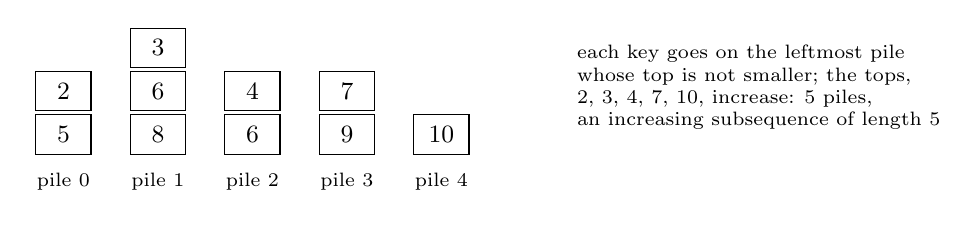
\begin{tikzpicture}[k/.style={draw, minimum width=7mm, minimum height=5mm, font=\small, inner sep=0pt}]
\foreach \x/\col in {0/{5,2}, 1/{8,6,3}, 2/{6,4}, 3/{9,7}, 4/{10}}
  \foreach \v [count=\r from 0] in \col \node[k] at (1.2*\x, 0.55*\r) {\v};
\foreach \x in {0,...,4} \node[font=\scriptsize] at (1.2*\x, -0.6) {pile \x};
\node[anchor=west, font=\scriptsize, align=left] at (6.4, 0.6) {each key goes on the leftmost pile\\ whose top is not
smaller; the tops,\\ 2, 3, 4, 7, 10, increase: 5 piles,\\ an increasing subsequence of length 5};
\end{tikzpicture}
\par\smallskip{\small Patience piles for $5, 2, 8, 6, 3, 6, 9, 7, 4, 10$: each pile grows upwards and never increases from
bottom to top. The number of piles is the length of a \omterm{def:b1:dynamic-programming:lis}{longest increasing subsequence}.}
\end{omfigure}

\section{Saving space}\label{sec:b1:dynamic-programming:space}

A row of the edit-distance table reads only the row above it: two rows suffice for the distance.

\omcode{code/bachelor-1/23-dynamic-programming/listings/edit_two_rows.py}{6}{14}{The \omterm{def:b1:dynamic-programming:edit}{edit distance} with two
rows}\label{lst:b1:dynamic-programming:two-rows}

\omoutput{code/bachelor-1/23-dynamic-programming/outputs/edit_two_rows.txt}{Two sentences: the same distance with 68
cells instead of 1258.}\label{out:b1:dynamic-programming:two-rows}

The price is the \omterm{def:b1:dynamic-programming:edit}{alignment}: the walk back needs the whole table. Hirschberg showed in 1975 how to recover it in linear
space anyway, by \omterm{def:b1:divide-and-conquer:dc}{divide and conquer}: compute the middle row of the table from the top with two rows, the same from the
bottom on the reversed words, find where an optimal \omterm{def:b1:dynamic-programming:edit}{alignment} crosses the middle row, and recurse on the two halves.
The time stays $\Theta(mn)$, about twice as much.

\section{Exercises}\label{sec:b1:dynamic-programming:exercises}

\begin{exercise}[$\star$]\label{exo:b1:dynamic-programming:1}
Fill the edit-distance table of \code{loan} and \code{lane}, and give an optimal \omterm{def:b1:dynamic-programming:edit}{alignment}.
\end{exercise}

\begin{exercise}[$\star$]\label{exo:b1:dynamic-programming:2}
How many calls do \code{fib_naive(6)} and \code{fib_memo(6)} make?
\end{exercise}

\begin{exercise}[$\star$]\label{exo:b1:dynamic-programming:3}
Add a sixth item of weight 3 and value 30 to the knapsack of \cref{out:b1:dynamic-programming:knapsack}: compute the new
row, and the items taken.
\end{exercise}

\begin{exercise}[$\star$]\label{exo:b1:dynamic-programming:4}
Find the length of a \omterm{def:b1:dynamic-programming:lis}{longest increasing subsequence} of $3, 1, 4, 1, 5, 9, 2, 6, 5, 3, 5$ with the piles, and one such
subsequence.
\end{exercise}

\begin{exercise}[$\star\star$]\label{exo:b1:dynamic-programming:5}
The one-row knapsack below goes through the capacities upwards or downwards. Explain the two results.
\omcode{code/bachelor-1/23-dynamic-programming/listings/exo_knapsack_up.py}{4}{10}{The knapsack on one row}
\omoutput[2-2]{code/bachelor-1/23-dynamic-programming/outputs/exo_knapsack_up.txt}{Items $(3, 25)$, $(4, 40)$, $(2, 15)$,
capacity 8.}
\end{exercise}

\begin{exercise}[$\star\star$]\label{exo:b1:dynamic-programming:6}
This memo is keyed on the identity of the list of values, which the recursion shortens and restores. Explain the wrong
counts and repair the key.
\omcode{code/bachelor-1/23-dynamic-programming/listings/exo_memo_mutable.py}{6}{18}{A memo keyed on a list}
\omoutput[2-4]{code/bachelor-1/23-dynamic-programming/outputs/exo_memo_mutable.txt}{Against all subsets.}
\end{exercise}

\begin{exercise}[$\star\star$]\label{exo:b1:dynamic-programming:7}
Talks $[s, f)$ now have weights. Find a set of compatible talks of largest total weight in $O(n \log n)$; the greedy rule
of \cref{thm:b1:greedy-proofs:earliest-finish} no longer works.
\end{exercise}

\begin{exercise}[$\star\star$]\label{exo:b1:dynamic-programming:8}
In how many ways can one climb $n$ stairs with steps of sizes taken from a given set, the order of the steps counting?
\end{exercise}

\begin{exercise}[$\star\star$]\label{exo:b1:dynamic-programming:9}
Show that the \omterm{def:b1:dynamic-programming:edit}{edit distance} equals the smallest cost of an \omterm{def:b1:dynamic-programming:edit}{alignment}.
\end{exercise}

\begin{exercise}[$\star\star\star$]\label{exo:b1:dynamic-programming:10}
Show another way that the number of patience piles is the length of a \omterm{def:b1:dynamic-programming:lis}{longest increasing subsequence}: each pile
never increases from bottom to top, and each key placed on pile $k > 0$ has a smaller key on pile $k - 1$ placed before it.
\end{exercise}

\begin{exercise}[$\star\star\star$]\label{exo:b1:dynamic-programming:11}
Compute the length of a longest subsequence of a word that is a palindrome, in $O(n^2)$, and test it.
\end{exercise}

\begin{exercise}[$\star\star\star$]\label{exo:b1:dynamic-programming:12}
With insertions and deletions only, show that the distance of $a$ and $b$ is $m + n - 2L$, where $m$, $n$ are their
lengths and $L$ the length of a \omterm{def:b1:dynamic-programming:lcs}{longest common subsequence}.
\end{exercise}

\section{Problem: A spelling checker for the catalogue}\label{sec:b1:dynamic-programming:problem}

\begin{problem}[{Weekend problem --- A spelling checker for the catalogue}]\label{pb:b1:dynamic-programming:1}
Eight misspelt queries are matched against the 80 titles of the catalogue, in lower case. The program computes \omterm{def:b1:dynamic-programming:edit}{edit
distances} with two rows, and avoids most of them with the triangle inequality: four titles serve as \emph{pivots},
whose distances to every title are computed once.
\omcode{code/bachelor-1/23-dynamic-programming/listings/spell.py}{24}{36}{The nearest title, with
\omterm{def:b1:backtracking:pruning}{pruning}}\label{lst:b1:dynamic-programming:spell}
\omoutput{code/bachelor-1/23-dynamic-programming/outputs/spell.txt}{Eight queries, their nearest titles, and the
distances computed.}\label{out:b1:dynamic-programming:spell}

\needspace{4\baselineskip}
\medskip\noindent\textbf{Part I --- The recurrence and its table.}
\begin{enumerate}
\item Why is the distance of \code{the silent comit} and \code{the silent comet} equal to 1?
\item How many cells has the table of a query of 19 characters against a title of 21?
\item In which order are the cells filled, and why is every cell read after it is computed?
\item What is the cost of one distance computation for words of lengths $m$ and $n$?
\item How many distances does a brute-force search compute per query?
\item Why is $D(i, 0) = i$?
\end{enumerate}

\needspace{4\baselineskip}
\medskip\noindent\textbf{Part II --- Alignments.}
\begin{enumerate}[resume]
\item Give an optimal \omterm{def:b1:dynamic-programming:edit}{alignment} of \code{the clokwork harbor} with \code{the clockwork harbour}.
\item Give two optimal \omterm{def:b1:dynamic-programming:edit}{alignments} of \code{catlaogue} and \code{catalogue}.
\item Why does the walk back always find a neighbour that gives the cell its value?
\item What is the cost of the walk back?
\item Why does the two-row version lose the \omterm{def:b1:dynamic-programming:edit}{alignment}?
\item Describe how the \omterm{def:b1:dynamic-programming:edit}{alignment} can still be found in linear space.
\end{enumerate}

\needspace{4\baselineskip}
\medskip\noindent\textbf{Part III --- Time and space.}
\begin{enumerate}[resume]
\item Read the cells kept by the full table and by two rows in \cref{out:b1:dynamic-programming:two-rows}.
\item How many cells does each version keep for two words of 1000 letters?
\item Does saving space change the time?
\item How many distances are computed once, for the pivots?
\item How many distances do the eight queries compute, against \omterm{def:b1:backtracking:exhaustive}{brute force}?
\item From how many queries on does the computation for the pivots pay off, at this rate?
\end{enumerate}

\needspace{4\baselineskip}
\medskip\noindent\textbf{Part IV --- A metric, and pruning.}
\begin{enumerate}[resume]
\item Show that $d(a, b) = 0$ exactly when $a = b$.
\item Show that $d(a, b) = d(b, a)$.
\item Prove the triangle inequality $d(a, c) \leq d(a, b) + d(b, c)$.
\item Deduce that $|d(q, p) - d(p, t)| \leq d(q, t)$ for any query $q$, pivot $p$ and title $t$.
\item Why can the loop stop at the first title whose bound is at least the best distance found?
\item State the named result, \emph{\omterm{def:b1:dynamic-programming:edit}{edit distance} is a metric}, with the saving it brings on the catalogue.
\end{enumerate}
\end{problem}
